\begin{tikzpicture}
\node [mybox] (box){%
    \begin{minipage}{0.3\textwidth}
    \txt{\footnotesize
        \begin{minipage}{0.5\textwidth}
            \textbf{Effet Doppler} variation de fréquence en cas de mouvement relatif entre la source et l'observateur.\\
            
            \textbf{Vitesse} relative de la source par rapport à l'observateur: $\vec{v}=\vec{v_s}-\vec{v_o}$
            
            $$f_o=f_s(\frac{\sqrt{1-(\frac{v}{c})^2}}{1+\frac{v}{c}cos(\theta)})^N$$
            {\footnotesize *N est le nombre d'allé-retour.}\\
            
        	\textbf{Effet transversale:} Si $\theta=90^\circ$ alors $f_o<f_s$\\
        	
        	\textbf{Déplacement Doppler}
            $$\Delta\lambda=\lambda_o - \lambda_s$$
            $$\lambda_o=\lambda_s (\frac{1+\frac{v}{c}cos(\theta)}{\sqrt{1-(\frac{v}{c})^2}})$$
            $$\frac{\Delta \lambda}{\lambda_s}=(\frac{1+\frac{v}{c}cos(\theta)}{\sqrt{1-(\frac{v}{c})^2}}-1)$$
            \textbf{Cas particulier}\\
            Si $\frac{v}{c}<<1$ ou $\frac{\Delta\lambda}{\lambda}<<1$ alors:\\
            $\frac{\Delta \lambda}{\lambda_s}=\frac{v}{c}cos(\theta)$
        \end{minipage}
        \begin{minipage}{0.35\textwidth}
            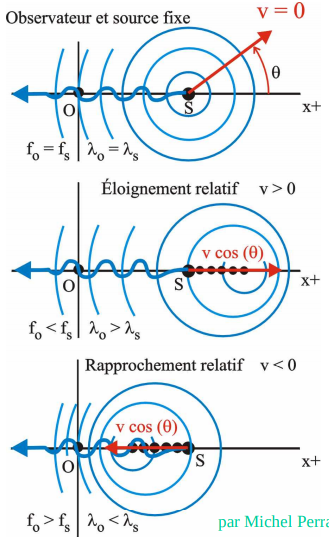
\includegraphics[scale=0.34]{images/effet_doppler.png}
        \end{minipage}
    }
    \end{minipage}
};
\node[fancytitle, right=10pt] at (box.north west) {Doppler};
\end{tikzpicture}